\chapter{Related Work}

Speech synthesis systems mostly use different electronic signal processing techniques to process speech signals. But people have been working on speech synthesis before electronic signal processing techniques. In beginning, people tried to build machines with mechanical devices which were used to create human sound. After the development of computers, better systems were built using different techniques. In \cite{swetha2013text}, basic speech synthesizing technique is discussed which works by concatenation of small recorded speech segments called phonemes to form complete speech. Words are first separated into syllables which is the unit that collectively depicts correct pronunciation of each word. Recorded speech of each syllable is then joined to get complete pronunciation of the word. The resulting voice needs some post processing as it has some delay due to concatenation of small units. These delays are removed in post processing which gives final pronunciation of the word. Preprocessing of the input text, guessing correct pronunciation of each word and prosody are the problems which make this system difficult. In preprocessing of text, all abbreviations and any type of numbers, time or dates are replaced with their corresponding text. Other issue is the speculating pronunciation of a word with respect to its context. For example, pronunciation of “lives” will be different in “He lives in Lahore” and “He saved two lives”. Stress and intonation is also most important and complex part of speech synthesis system which is necessary for naturalness in synthesized speech. A text to speech (TTS) system for Azerbaijani language is developed using concatenative synthesis in \cite{aida2010main} where small recordings were concatenated to make speech waveform.

In \cite{liberman1992text}, two sub parts of TTS system, text analysis and word pronunciation, were discussed. TTS system is divided in 4 sub parts: text analysis, word pronunciation, phonetic interpretation and signal generation. Text analysis step includes division of text into sentences, words, phrases and expansion of abbreviations etc. Text analysis is required to get correct context and pronunciation of each word in a sentence. In text analysis, sentence division and parts of speech tagging is done by using heuristic solutions \cite{riley1989some} and dynamic programming respectively. For word pronunciation, dictionary based approach was used for about 99.9\% words and for 0.1\% words, letter to sound rules were followed. 

A technique based on letter to sound rules is also developed in \cite{elovitz1976automatic}. Total 329 letter to sound rules have been created. These rules take text as input and translate it into phonetic alphabet which in turn converted to synthetic sound. This system produces about 97\% correct pronunciation of phonemes. The paper also describes software and hardware requirements and overall performance statistics of this system. The dataset is developed by extracting 50,000 words from Brown corpus \cite{ku1967computational}. The system gave accuracy of about 93\%. A more improved system was proposed in \cite{carlson1982multi, klatt1982klattalk}. In \cite{klatt1982klattalk}, a TTS system is developed for English and simple numerical and algebraic expressions. The system is rule based system having 500 letter to sound rules. However, it can use pronunciation dictionary of 1500 words for exceptions. The system interface provides facility of selection of voice types (Male or Female). The word boundaries and probable position of phrases and clauses is analyzed by syntactic analyzer. The phonemes of word are then passed to synthetic speech synthesizer that converts phoneme to sound by following extensive set of rules and rules for consonant-vowel transitions. The whole process is divided in two sub processes, text analysis which is conversion of text to corresponding linguistic representation that comprises of phoneme, stress and boundaries and positions of respective vowel or consonant and durational phenomena such as pauses, interaction between segments \cite{klatt1979synthesis} and speech synthesis in which sequence of phonemes are converted to speech sound with the help of some set of rules. The abbreviations in input data are converted to their respective text and if dictionary does not have their respective words, the abbreviation is pronounced as a word. After preprocessing, the words are exposed to letter to sound rules. If an unstressed function appears in text and there is no rule for it then it is passed to pronunciation dictionary. The results show that about 95\% rules were successful when executed. The syntactic analyzer then determines the structure of sentence according to its pauses and boundaries. The phoneme to speech rules are divided into two components, phonological that provide information of stress and rhythm and duration of words in a sentence. All these outputs are then passed to synthesizer that produces synthetic sound. Synthesizer is simple version of synthesizer proposed in \cite{klatt1980software}.

In \cite{carlson1982multi}, TTS system is presented which require some hardware resources as well with the enhancements in microprocessor, memory and signal processor technology. This TTS system can be put into portable form and can be used anywhere with different systems. A higher level language is developed in laboratory that can be easily used for linguistic processes. These enhancements and developments in hardware and software level made transforming of text to speech at 250 wpm rate. This combination of hardware and software is tested against several applications used for handicaps. The fundamental reason for this framework is to make a system that will be utilized for transformation of any language from text to speech. 

In \cite{huang1996whistler}, Whistler which is a TTS engine is developed by using prosody and concatenative speech parameters that were extracted using probabilistic learning methods. The resulting voice of this TTS system appears to be very much real. This system can also help to build TTS system for other languages.

A formant and concatenative synthesis is developed in \cite{huang1997recent} where small segments of phonemes were concatenated to form whole speech. A recorded speech database of about 6,000 phonetically balanced sentences is used for training of the system. The technique which has been used in Whistler \cite{huang1996whistler} can significantly encourage the way toward making bland TTS system for new speech style. This system supports Microsoft Speech API \cite{ms_speech_api} and requires under 3 MB memory.

In \cite{hunt1996unit}, linear regression and unit selection based speech synthesis is designed using ATR Japanese database. In this algorithm, raw text is converted to phonetic strings and against each phoneme, best candidate unit from a huge database of speech units is selected with \textit{Viterbi} search. By concatenating these units, target waveform is generated. These units can be contemplated as state transition network where each unit represents a different state. The cost of the system depends on target cost and cost of the concatenation of units. Each phoneme and unit is denoted by a multi-dimensional feature vector. Weighted difference of target and candidate feature vector is taken in order to measure the target cost. Similarly, the cost of concatenation is also measured by weighted sum of sub-cost of concatenation. Cost function can be trained in two different ways. In Weight Space Search method, units are searched with \textit{Viterbi} and distance between constructed waveform and natural waveform is minimized. In Regression Training, linear regression is used to choose best unit from the list of all possible units for a given phoneme.

Statistical parametric speech synthesis is another approach which is gaining popularity in recent couple of years \cite{king2010beginners}. This approach works better than concatenative technique on smaller data. On larger data, concatenative synthesis can produce better quality speech. In this technique, HMM or model firmly related to HMM are used for training model over given data. HMM based statistical parametric speech synthesis has picked up notoriety as a result of its capacity to produces top notch speech automatically with parametric flexibility, less data and resources \cite{black2007statistical}.

A multi-dimensional Gaussian distribution based HMM based statistical parametric speech synthesis system was developed in \cite{yoshimura1998duration}. In this approach, duration models clustering is performed using decision tree based context clustering. The contextual factors are also considered with phone identity factors. Mel-cepstral coefficients are calculated and model is trained by these coefficients. Context clustering technique which is based on decision tree is used for clustering of the context dependent HMMs \cite{odellj.j1995}. In state duration modeling, multi-dimensional Gaussian distributions are used to model HMM. The clustering of the duration models is performed after estimation using clustering technique based on decision tree. By traversing decision tree, all contexts can be searched. Contextual factors which effects timing of events in speech are also taken into account and resultant speech shows that it has good quality and natural timing. For testing of the system, 450 sentences of Japanese are used for training of system. Sampling of speech signal is done at 16 kHz. Feature vector is composed of 25 mel-cepstral coefficients. There were 3030 states and 2984 distributions in output of the system. The listening tests show that synthesized speech has good quality.

A similar system is designed in \cite{tokuda2000speech} using HMM and evaluated by taking input from Japanese database. The parameters in this system are generated with HMM. The state sequence fully or partially is hidden due to which iterations are performed for parameter generation and forward-backward algorithm is used for the situation where state sequence is provided. This algorithm, from multi-mixture HMMs, can generate clear formant structure.

A HMM and unit selection based system is proposed in \cite{tokuda2002hmm} where model is trained with speech database after which excitation and spectral parameters are calculated. These extracted parameters are modeled by context dependent HMMs. Decision tree based context clustering technique is used in order to get correct model parameters which are then used in speech synthesizer for generating speech signals. The speech characteristics can be controlled using these parameters. In \cite{harashima2006review}, HMM and rule based approaches are applied on voices taken from e-learning courses and online lessons for dataset creation and tested by generating voices and given as input to students to interpret it.

Corpus based approach for Expressive Prosody Modeling is applied in \cite{eide2004corpus} where manually produced dataset was used. To evaluate the synthesized
speech and expression, the output is given for testing to 32 native English speakers. Test is performed with different types of sentences like bad news, good news and for yes/no and the accuracies we get are 70.2\%, 80.3\% and 84\% respectively.

% Tones and Break Indices ToBI are discussed on American English in \cite{pitrelli2004tobi}. Majorly
% bi-gram and tri-gram were used to predict the occurrences of particular word or letter. Analysis
% was performed by multiple techniques. The corpus was divided into following five yes-no
% questions, either-or questions, other questions (hereafter, “wh-questions”), exclamations, and other
% declarative sentences categories for the analysis purpose. Analysis by word frequency count
% produced not good results and the reason was that the data was of variant types. The results show
% that professional speakers produces better and informative prosodic events as compared to
% ordinary speakers.

HMM based approach is used in \cite{baloyi2012text} to construct a speech synthesizer for Xitsonga which is an African language. The dataset used here consists of phone set of consonants and vowels. These sets utilized to set up a set of letter to sound rules to be used in TTS system. The main tool used for speech synthesis is HTS toolkit \cite{hts_2.2} with other software that support to setup complete environment for speech synthesis. HMM based approach is used in this study because HMM based statistical parametric speech synthesis can be used to synthesize speech waveform without requiring huge dataset for training. The system received acceptability of 92.3\%. 

TTS system is designed in \cite{dagba2014text} for Fon language using Multisyn algorithm \cite{clark2007multisyn} which consists of Natural Language Processing (NLP) and Digital Signal Processing (DSP) modules. NLP consists of segmentation, Letter-to-Sound conversion and back-off rules module. When a character is not found in known characters' list, back-off rules are applied. DSP module than choose required unit from database of units are concatenate them to form complete speech signals.

In \cite{ganai2016text}, hybrid TTS converter is developed by concatenating benefits of HMM and waveform based TTS system. For developing it, an audio phoneme library is used. The main edge of developed system over other is that it produced more human like voice/speech. The experiments were taking in Matlab and a phoneme library is developed that consists of audio files and dictionary of words with their phoneme. Sentence is taken as input then model parsed it into words. The system analyzes each word, gets its phoneme and combines all phonemes and plays the sound. Waveform for each sound is also presented. This sub-ban speech synthesized approach is obtained by this combination of models that improved the quality of synthesized speech. The quality of speech is not good enough, in future system will be improved to get better controls.

A speech synthesis system is introduced in \cite{donovan1995improvements} which uses context-dependent HMM for defining set of subphone units. This system uses context-dependent HMM for defining set of subphone units. These subphone units are then used in concatenation synthesizer. The training data is one hour recorded speech which is used for getting required parameters. TD-PSOLA waveform concatenation synthesizer is then used to generate pronunciation using these parameters. The synthesized speech is very natural and intelligible. This system uses automatic statistical processes to extract segments of speech from large speech carpus. Desired sentence is produced by concatenation of small segments of speech. HMM is trained and used for segmentation of speech database into HMM-state-sized units. A decision tree is constructed by using phonetic context labels which is used for clustering of the training speech into acoustically self-comparable grouped states. This process helps to find most important context effects. The string to be converted into speech is first converted into sequence of phonetic strings which then using decision tree is changed over to speech segments which are used to generate final speech signals. Modified Rhyme Tests \cite{house1965articulation} were used to compare system with other. Six listeners were used with each give an answer sheet, and they have to mark word from list of provided words which is played during test. The MRT error rate for test was 5.0\% and standard error rate was 0.47\%. HMM is used for training of the model. The dataset used for training of model is recorded speech. Four datasets are used in which are termed as M2, M3, F1 and F2 where M stands for male and F stands for female. Six listeners evaluate output produced by model. The MRT error rate and standard error rate for test was 5.0\% and 0.47\% respectively. In future, segment selection algorithm used in the system can be improved where segments in each state would be available in speech synthesis process. The process of searching optimal segment sequence can be improved by using dynamic programming.

\cite{masuko1996speech} present a TTS system which is based on HMM which comprises dynamic features. Speaker adaptation technique \cite{tamura1998speaker} and speaker interpolation technique \cite{yoshimura2001speaker} can be used to modify voice characteristics of speech in statistical parametric speech synthesis system. The HMM based statistical parametric TTS system can model speech parameters like spectrum or excitation with the help of context-dependent HMM and construct speech signals. Version 2.0 of already build HMM based TTS system (HTS) toolkit is presented in \cite{zen2007hmm}. HMM based speech synthesis system can build speech synthesis system even with small dataset for training \cite{huang2001spoken} but the quality of that speech will not be equal to recorded speech. 

% In \cite{merritt2013investigating}, author discussed shortcomings of Hidden Markov model and majorly focused on the findings that HMM based TTS system are not better than simple concatenative TTS systems. Experiments performed and then through pairwise listening test, the HMM based system is evaluated. Based on the responses of qualities, model molded to tackle further situational problems. In figure \ref{fig:Merritt_tts}, architecture of this system is shown.
% \begin{center}
% 	\begin{figure}[hbtp]
% 		\centering
% 		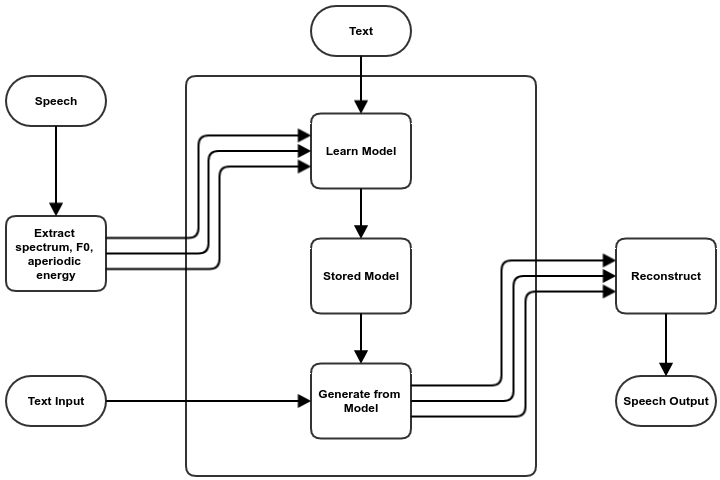
\includegraphics[width=\linewidth]{images/Merritt_tts.png}
% 		\caption{TTS System Architecture using HMM speech synthesiser}
% 		\label{fig:Merritt_tts}
% 	\end{figure}
% \end{center}

% Experiments show that when variance is too high then smoothing has a beneficial effect as it
% reduces the variance and bring the points closer to the natural one. For future, needs to work over spectral envelope over-smoothness, averaging across multiple tokens of similar speech sounds, model boundary discontinuities in the trajectory and
% inconsistencies between the different speech parameter streams \cite{merritt2013investigating}.

A more advance technique is Neural Networks based technique as it works better than HMM based technique. Time domain Neural Networks with database containing sounds of words called phonemes is used in \cite{karaali1998text}. The basic flow of the system involves speech recording, speech labeling, voice coder and input processing using Time Delay Neural Network. The figure \ref{fig:Time Domain Neural Networks based TTS System} shows the block diagram of system.

\begin{center}
	\begin{figure}[hbtp]
		\centering
		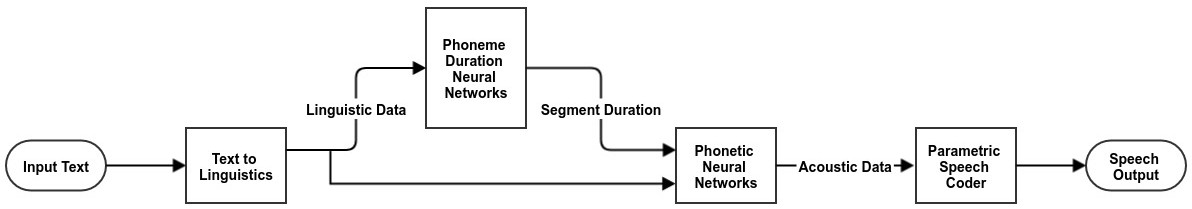
\includegraphics[width=\linewidth]{images/time_domain_neural_network.jpg}
		\caption{Time Domain Neural Networks based TTS System}
		\label{fig:Time Domain Neural Networks based TTS System}
	\end{figure}
\end{center}

Neural Networks based techniques are used to learn features automatically during training along with the combination of various techniques like linear regression and Neural Networks in \cite{yoshimura2016hierarchical}. Dataset of all previous Blizard Challenges \cite{blizzard_2009_corpus} and afterwards up to 2013 were used. Model was evaluated using 5-fold cross validation. The given model gave 0.11\% and 0.17\% error for LR+LR and LR+NN respectively. Neural Networks is also used in \cite{wu2016merlin} with dataset consisting of 328 hours which was collected in voice of native 1506 speakers. The model is tested by giving 20 sets of randomly selected from evaluation set and asked them to rate output of each set between 0 and 100.

Deep Neural Networks is applied in place of HMM in \cite{ze2013statistical} as HMM based system cannot model complicated context dependencies. There are impediments in HMM based system that Deep Neural Networks (DNN) can cover and also likewise beat HMM based system. 

Recurrent Neural Networks (RNN) is applied in \cite{fan2014tts} by using the Bidirectional Long Short Term Memory (BLSTM) with dataset consisting of 5000 training utterances and 200 utterances for testing the system. Whole recording was done in voice of the female native speaker. Objective and subjective evaluation measures are used to find distortion between natural and synthesized speech and quality respectively which shows that hybrid system is better as it gave 44\%, 59\% and 55\% accuracy whereas the Neural Networks, HMM and DNN gave 29\%, 22\% and 20\% accuracy respectively. In \cite{muthukumar2016recurrent} Recurrent Neural Networks (RNN) postfilters are used for speech synthesis. 

Researchers have also been working on TTS system for Urdu language for many years. A bi-lingual TTS synthesis 
system for Urdu and Sindhi is designed in \cite{shah2004bi} using bilingual hybrid knowledge based approach by using concatenated synthesis method which is capable of providing high quality Urdu and Sindhi speech. This system can be further expanded to include sensitive and visual text-to-speech (VTTS) policies in future.

In \cite{ahmed2014hmm}, an HMM based speech synthesis system is developed for Urdu. The speech corpus is created by recording 1 hour and 15 minutes of speech containing 989 sentences in total. In training phase, context level and prosody level parameters are extracted from recorded sentences e.g. counts, position, distances, stress and phone utterance information. F0 excitation parameter and mel-cepstral coefficients are calculated using RAPT \cite{kleijn1995speech}. The F0 is modeled using frequency distributions discrete for unvoiced and continuous for voiced regions. These HMM models are then clustered using decision trees. In text analysis, numerals and abbreviations in input text are preprocessed and converted to full textual forms. The date/time and numeric notations are processed using regular expressions (rule based component) and abbreviation are converted to text by finding their corresponding words from dictionary. This stage is followed by diacritic restoration stage which used dictionary develop by CRULP \cite{crulp} to restore diacritics. After this, G2P converter which follows guidelines of \cite{hussain2004sound} is used to convert grapheme to phoneme. In synthesis module, input text is labeled and then by speech synthesis algorithm, it generates speech features which are passed to filter and obtain speech signal. The model uses 36 consonants and 10 vowels. All speech recordings in a corpus are converted to their phoneme representation and saved in pronunciation dictionary after checking by author. After this, STRAIGHT vocoder is used to estimate speech parameters and generation of speech waveform. 680 questions were gathered by using spectrum and context features, speech parameter were generated using maximum likelihood criteria. For evaluation of system, the author listened to synthetic speech himself and found that it is not intelligible but can be improved in future work.

In \cite{nawaz2014hidden}, a TTS system for Urdu is developed by using HTS toolkit and Urdu Qaida of grade 2 and 4. This system consists of two processes, text analysis and synthesis of speech. Here feature extraction and calculation of mel-cepstral coefficient is done using technique mentioned in \cite{fukada1992adaptive}, text processing is done using \cite{kabir2002natural} and process of synthesis using process described in \cite{tokuda2000speech}. The HTS toolkit is available for English, Japanese and Portuguese languages. For Urdu, certain modifications are needed which involve creation of context level labels and questions file for Urdu phoneme set. Frequently speaking Urdu words were identified by using greedy algorithm and question files are made to deal with the issue of data sparsity as in a model, only a certain amount of examples can be handled during training phase. If we look on to the contextual level, it is observed that multiple contextual occurrences exist for a single phoneme. To deal with this problem, a clustering method is used to cluster similar acoustic words. The whole training set is placed into single cluster and on the basis of each question, cluster is split. The cluster is chosen on the basis of the question which minimizes the objective function. In the evaluation process, experiment is performed by using 200 frequent Urdu words and native Urdu speakers. Testing of the system shows that the system gives output which is intelligible but not very natural. The reason behind this is data used in training phase consists of full sentences rather than words. Performance with respect to naturalness can be improved by using words instead of sentences because of clarity and length of word. It is found that 92.5\% words are correctly identified. The system has taken 66 phonemes but for better performance at least 270 examples should provide the system during training phases.

Natural Language Processing unit is very importing unit in speech synthesis system as it handles all language related issues. This unit performs a list of steps for its complete operation which contains tokenization, semantic tagging, string generation, syllabification, stress and intonation marking etc. \cite{saleem2002urdu, urdu_text_preprocessing} discuss such unit for Urdu language. This unit is divided in two parts called as preprocessing and phonological processing unit. Preprocessing unit process all numbers, dates and time in input data and converts them into their respective words. For example, 1000 and 6-10-2012 will be changed into \texturdu{ہزار} and \texturdu{چھے اکتوبر دو ہزار بارہ} respectively. All special characters like \$ and & are also processed in this unit. In last step of preprocessing unit, data is passed through grapheme to phoneme converter. In phonological processing unit, syllable boundaries, stress and intonation are marked by their respective markers.

% A speech corpus is developed using 10 hours recorded speech of professional speaker containing of 1036 sentences in \cite{mumtaz2016break}. Globalphone which is a database of multilingual types is elaborated in \cite{schultz2002globalphone}. This
% database contains high quality voice vocabulary which can be used for voice recognition and text to speech system. It
% contains dataset of consisting more than 300 hours in voice of 1500 native speakers. It mainly cover English, Arabic,
% Japanese, Turkish and 11 more languages. Scientific work done on Urdu language is limited mainly due to the reason that
% there is not enough material related to phonetic strings are available for Urdu. 

% In \cite{urdu_tts_db_kashif2015}, Neural Networks consists of feed forward network, back propagation for weight updation is used to generate 
% speech synthesis system for Urdu. An interface is designed and tested. Mean Square Error of designed system is used as performance parameter. 
% The MSE is 0.00867 of proposed system. A large database consists of 59 Urdu characters, vowels and numbers is created for this system. The designed model only
% produces synthetic sound of single character. In future, urdu sentences are added to generate output in the form of full text.

\cite{saleem2002urdu} discussed consonantal and vocalic sounds for Urdu Language in detail. In \cite{hussain2005phonological}, phonological processing unit for Urdu language is discussed in detail. In this module, word boundaries are marked by tokenizer which is called text normalization. This is followed by marking of syllable boundaries by using letter to sound rules. The syllabified data is processed to apply sound change rules. This is followed by stress and intonation marker. In \cite{anwar2007statistical} a statistical based part of speech tagger for Urdu language is discussed which works by calculating probability of each word given a particular tag. Unigram model assign tag for each token that has the maximum probability. Conditional probability for given tags against each word using maximization principle as used in \cite{bird2007introduction}, \cite{carlberger1999implementing}. The model is evaluated by comparing Unigram, Bigram and Backoff experiments with different size of tag sets. t-test, POS accuracy are used to measure performance. Bigram model considered maximum likelihood principle keeping an eye on the context of text. Backoff model was used to blow away sparse problems. Problems in Urdu segmentation are discussed for Urdu in \cite{durrani2010urdu}. Clause boundary identification is discussed in \cite{parveen2011clause} using clause markers and classifier in Urdu language using conditional random field as a classifier.

% In \cite{anwar2007statistical} small tagset was
% comprised of 90 tags and large of 250 tags. They applied tags out of all possible tags for a particular word set accurately. It
% gave

% \begin{itemize}
% 	\item 94.3\% accuracy for small tag set when Unigram model is used
% 	\item 88.50\% accuracy for small tag set when Bigram model is used
% 	\item 95.00\% accuracy for small tag set when Backoff model is used
% 	\item 91.10\% accuracy for large tag set when Unigram model is used
% 	\item 83.70\% accuracy for large tag set when Bigram model is used
% 	\item 91.65\% accuracy for large tag set when Backoff model is used
% \end{itemize}

% Overall method was 95\% efficient. Data was not automatically tagged in \cite{anwar2007statistical} rather it was tagged by human
% intervention. There is larger gap for accuracy to be higher using some other methods of training data.


% Concatenative speech synthesis is the model of speech synthesis where waveform is generated using concatenation of small units. In \cite{lemmetty1999review} the process of speech synthesis is divided into High-level and Low-level synthesis. In High-level, text is converted into phonetic strings. Low-level synthesis process is done by Articulatory, Concatenative and Formant based synthesis. In formant based speech synthesis, resonances in the vocal tract is modeled and this technique was widely used in
% past. In concatenative synthesis, prerecorded speech samples are concatenated to form complete speech signals \cite{pickett1999acoustics}.

% This IBM Expressive TTS System amazingly produced good results not only on neutral sentences and conditions but also
% including good news, bad news and questions. In addition to this SSML made it capable for end users to add their customized
% expressions to our system. Based on desired expressions in sentences the final audio output includes those expressions for
% conveying meaningful messages.


\section{Discussion}
Raw text can be converted into speech by concatenation of small units of speech from a huge single-speaker speech database. Huge database makes it possible to produce more natural sound. TTS system development can be based on rules for generation of speech but this method can take intensive labor and rules are difficult to be general so that they can be used for other languages as well. In prosody modeling, linguistic rules are used \cite{klatt1987review, pierrehumbert1981synthesizing} but speech produce by this approach felt to be robotic. So in order to increase quality of voice, large units are used. This strategy enhanced naturalness as well as diminished expected time to create new voice and furthermore made the manufactured speech like unique benefactor speaker.

The best approach for speech synthesis until now is considered to selection synthesis but it has certain limitation that is it need large database of recording which is very expensive and not feasible for certain languages \cite{black1994chatr, hunt1996unit, black2003unit}. Statistical parametric speech synthesis is becoming popular and being used for number of languages like English \cite{tokuda2002hmm}, Chinese \cite{qian2006hmm}, Arabic \cite{abdel2006improving}, Croatian \cite{martincic2006croatian} and Urdu \cite{ahmed2014hmm}. The advantage of parametric over selection is that it does not require saving original signal for synthesis due to which database is small for this approach \cite{zen2009statistical}. Basic TTS system focus over conversion of text to voice using multiple techniques \cite{merritt2013investigating}. Different synthesis model has been developed but HMM is becoming popular from last few years \cite{ze2013statistical}. There are multiple tools for TTS but freely available tools mostly use 2 techniques i.e.

\begin{enumerate}
	\item HMM based speech synthesis called SPSS
	\item Simple waveform concatenation.
\end{enumerate}

SPSS technique is attractive although its results are comparatively not amazing. In recent years, the use of statistical modeling in speech recognition system has increased a lot and most of these systems are using HMM for acoustic modeling of the system \cite{donovan1999hidden}. These systems enable us to construct models with large amount of data that is difficult to analyze manually. This technique can be applied on the process of speech synthesis. This type of system can be used to run on different data, voices and languages \cite{donovan1999hidden}. There are many TTS systems which are capable of generating high quality speech, but they cannot generate speech with different speaking style and voice because speech data required by these systems in order to get these characteristics is very large. HMM based speech synthesis system \cite{tokuda2002hmm} is capable of doing this without needing large speech database. A speech synthesis system can be developed using statistical learning techniques. These systems can be trained and voice characteristics of original speaker can be produced in synthesized speech. This type of system can be built with HMM and its performance can be improved by techniques like context-dependent modeling and environment adaptation techniques \cite{tokuda2000speech}. It has many advantages like ability to change voice characteristics and robustness which will be very difficult in concatenative speech synthesis. But it has some limitations like inefficiency in handling complicated context ascendance \cite{ze2013statistical}.

Another famous speech synthesis approach is unit selection in which small units of recorded speech are concatenated in order to synthesize speech waveform. This technique can generate high quality speech signals but for getting various characteristics of synthesized speech, a huge database is required. On the other hand, this can be achieved using HMM based statistical parametric TTS system without needing large speech database \cite{zen2007hmm}. A considerable measure of research chip away HMM approach but the output voices produced by these kinds of systems look unnatural sometimes. It is surprising that by the time this should be improved a lot but there are still existing problems and drawbacks that decrease the performance of TTS system, as compared to other simpler concatenation based TTS systems. Through literature review it is easy to say that HMM system do over smoothing which cause unnaturalness for TTS System output. There is no proper study which can prove this hypothesis so \cite{merritt2013investigating} present the reasons for this unnatural behavior \cite{merritt2013investigating}.

Many TTS systems have been purposed and each have its own pros and cons. For example, waveform based model is good enough to produce human like sound but it requires large database. In rule based techniques, most of the time rules updating is required and novelty is too much difficult with traditional rules. Similarly, with concatenation of phonemes, it is also difficult to bring novelty and handle new and unseen words \cite{karaali1998text, pitrelli2004tobi}. Neural Networks can be used to improve results of speech synthesis system \cite{muthukumar2016recurrent}. From recent years, Neural Networks are being used as acoustic models \cite{ling2015deep, zen2015acoustic}. There exists a wide research over the correlation between acoustic modeling and linguistic features in late 90s \cite{cawley1993lsp}. Now more focus is not Neural Networks based techniques. Neural Networks easily map linguistic features to acoustic models using feed forward approach \cite{lu2013combining, qian2014training, chen2015deep, ze2013statistical}. 